% !TEX TS-program = pdflatex
% !TEX encoding = UTF-8 Unicode

% This file is a template using the "beamer" package to create slides for a talk or presentation
% - Giving a talk on some subject.
% - The talk is between 15min and 45min long.
% - Style is ornate.

% MODIFIED by Jonathan Kew, 2008-07-06
% The header comments and encoding in this file were modified for inclusion with TeXworks.
% The content is otherwise unchanged from the original distributed with the beamer package.

\documentclass{beamer}
\setbeamercovered{invisible}



% Copyright 2004 by Till Tantau <tantau@users.sourceforge.net>.
%
% In principle, this file can be redistributed and/or modified under
% the terms of the GNU Public License, version 2.
%
% However, this file is supposed to be a template to be modified
% for your own needs. For this reason, if you use this file as a
% template and not specifically distribute it as part of a another
% package/program, I grant the extra permission to freely copy and
% modify this file as you see fit and even to delete this copyright
% notice. 


\mode<presentation>
{
  \usetheme{Warsaw}
  % or ...

  % or whatever (possibly just delete it)
}


\usepackage[english]{babel}
% or whatever

\usepackage[utf8]{inputenc}
\usepackage{qrcode}
\usepackage{hyperref}
\usepackage{ytableau}
\usepackage{longtable}
% or whatever

\usepackage{times}
\usepackage[T1]{fontenc}
\usepackage{tikz}
% Or whatever. Note that the encoding and the font should match. If T1
% does not look nice, try deleting the line with the fontenc.

%%% MATH RELATED

\title{MATH 180 Strategies of Problem Solving} 
\subtitle
{} % (optional)

\author[W.R. Casper] % (optional, use only with lots of authors)
{W.R. Casper}
% - Use the \inst{?} command only if the authors have different
%   affiliation.

\institute[California State University Fullerton] % (optional, but mostly needed)
{
  Department of Mathematics\\
  California State University Fullerton}
% - Use the \inst command only if there are several affiliations.
% - Keep it simple, no one is interested in your street address.

\subject{Talks}
% This is only inserted into the PDF information catalog. Can be left
% out. 



% If you have a file called "university-logo-filename.xxx", where xxx
% is a graphic format that can be processed by latex or pdflatex,
% resp., then you can add a logo as follows:

% \pgfdeclareimage[height=0.5cm]{university-logo}{university-logo-filename}
% \logo{\pgfuseimage{university-logo}}



% Delete this, if you do not want the table of contents to pop up at
% the beginning of each subsection:
\AtBeginSubsection[]
{
  \begin{frame}<beamer>{Outline}
    \tableofcontents[currentsection,currentsubsection]
  \end{frame}
}


% If you wish to uncover everything in a step-wise fashion, uncomment
% the following command: 

%\beamerdefaultoverlayspecification{<+->}


\begin{document}

\begin{frame}
  \titlepage
\end{frame}

\begin{frame}{Outline}
  \tableofcontents
  % You might wish to add the option [pausesections]
\end{frame}

% Since this a solution template for a generic talk, very little can
% be said about how it should be structured. However, the talk length
% of between 15min and 45min and the theme suggest that you stick to
% the following rules:  

% - Exactly two or three sections (other than the summary).
% - At *most* three subsections per section.
% - Talk about 30s to 2min per frame. So there should be between about
%   15 and 30 frames, all told.

\section{SoPS Lecture 19}

\begin{frame}{Review}
  \begin{block}{Last time}
    \begin{itemize}
\pause
      \item Sets, Subsets, Intersection, Union, Complements
\pause
      \item Cardinality of finite sets, power set
\pause
      \item Universal quantifiers, Russell's paradox
    \end{itemize}
  \end{block}
\end{frame}

\subsection{Functions}

\begin{frame}{Intuition}
\begin{center}
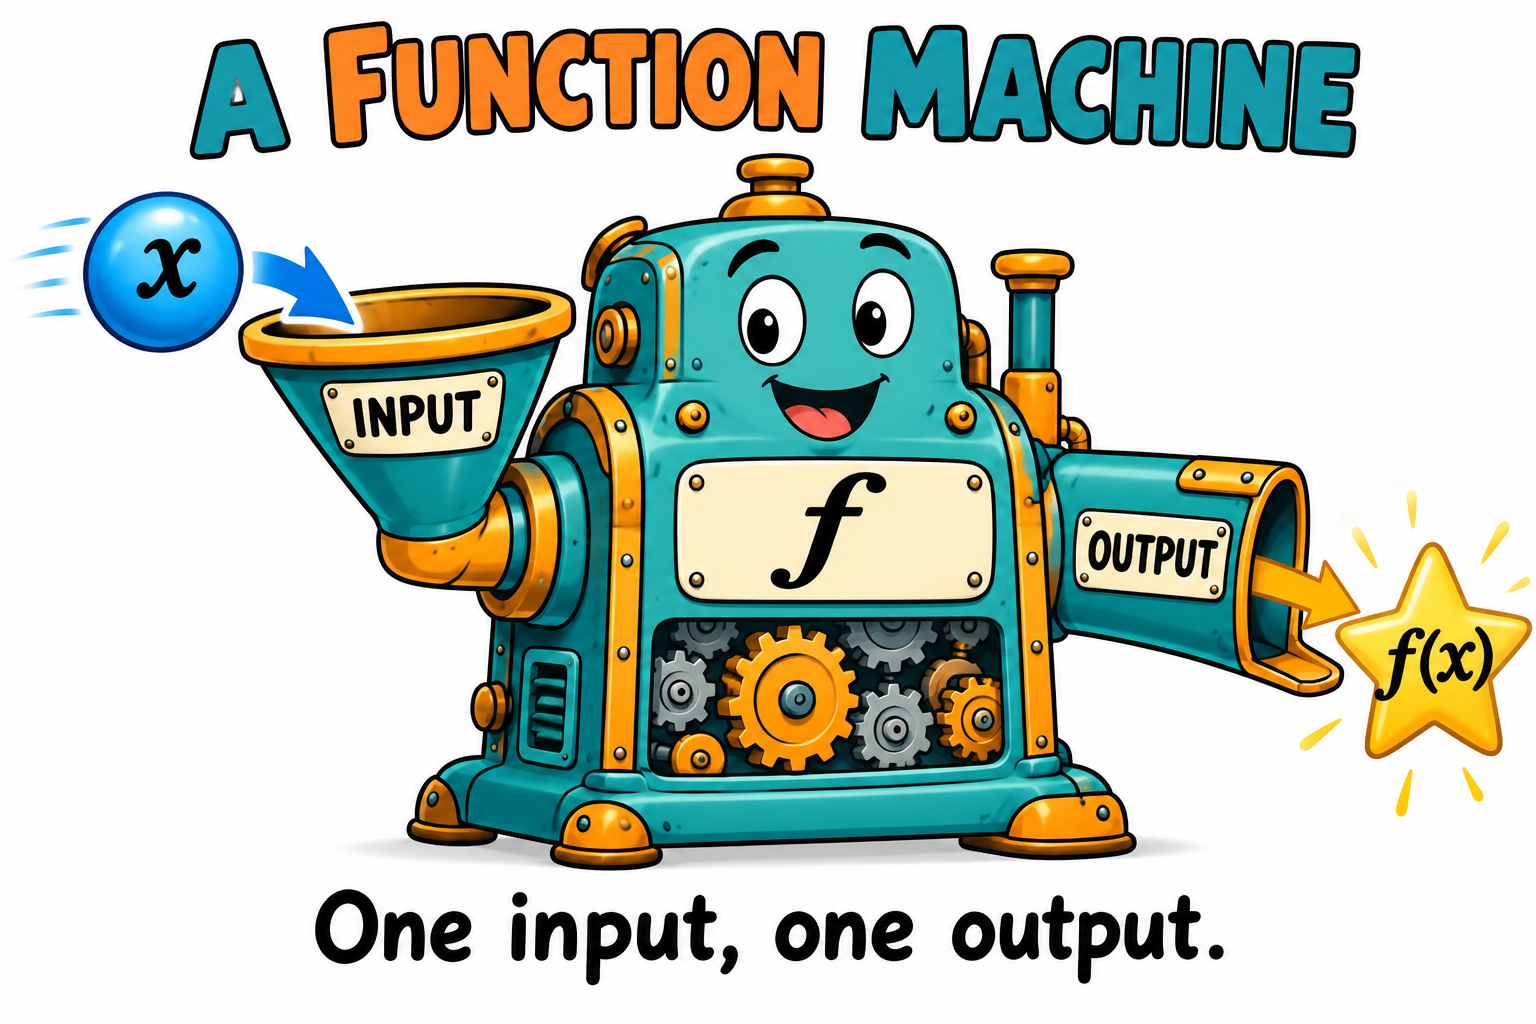
\includegraphics[width=0.8\linewidth]{fig/fun1}
\end{center}
\end{frame}

\begin{frame}{Intuition}
\begin{center}
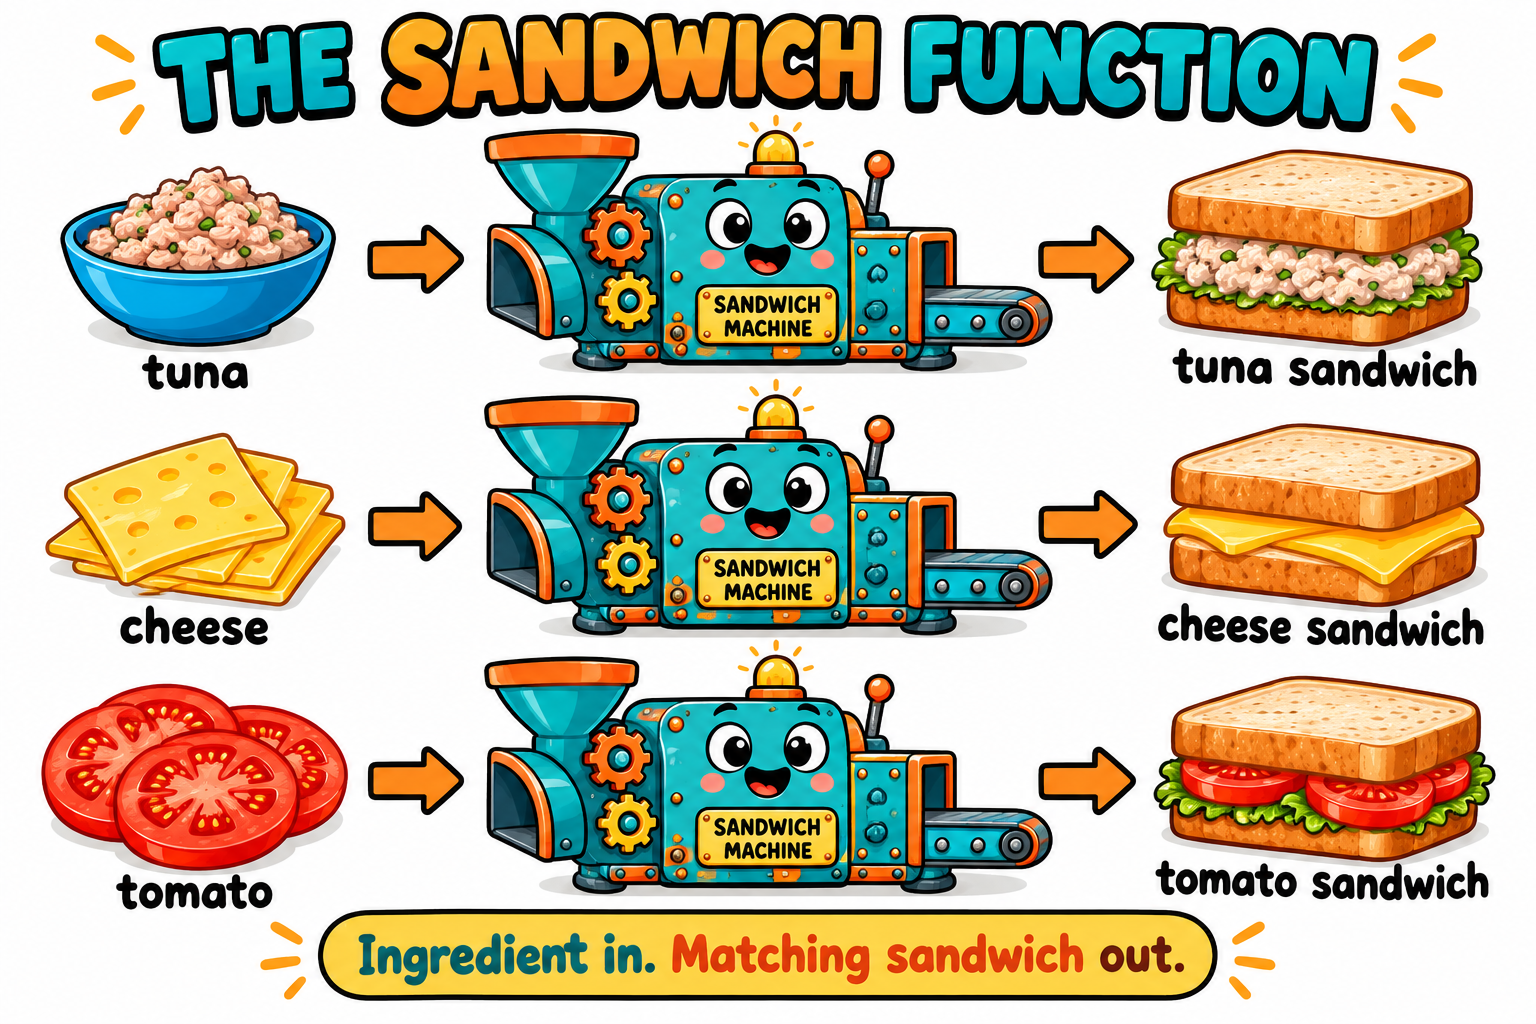
\includegraphics[width=0.8\linewidth]{fig/fun2}
\end{center}
\end{frame}

\begin{frame}{Intuition}
\begin{center}
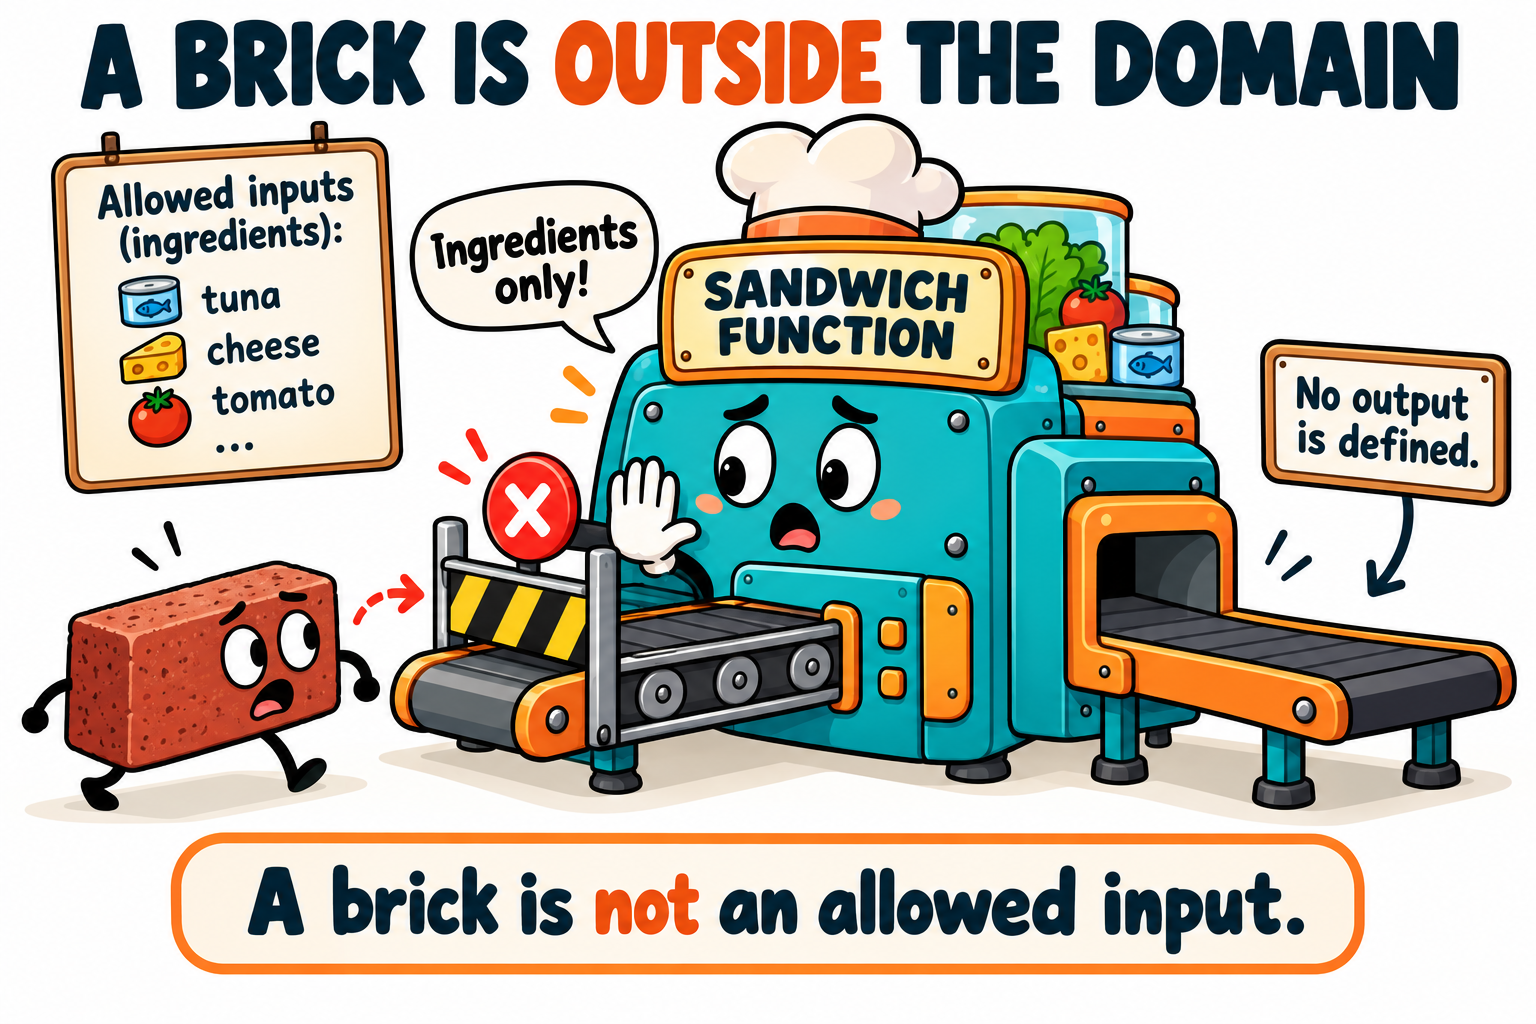
\includegraphics[width=0.8\linewidth]{fig/fun3}
\end{center}
\end{frame}

\begin{frame}{Relations}
\pause
\begin{block}{Definition}
A \textbf{relation} $\mathcal R$ from $A$ to $B$ is a subset of the Cartesian product $A\times B$.\\
\pause
The \textbf{domain} and \textbf{range} of $\mathcal R$ are
$$\text{Dom}(\mathcal R) = \{a\in A: \exists b\in B,\ (a,b)\in\mathcal R\}$$
$$\text{Rng}(\mathcal R) = \{b\in B: \exists a\in A,\ (a,b)\in\mathcal R\}$$
\end{block}
\end{frame}

\begin{frame}{Relations}
\pause
\begin{block}{Example}
\pause
$$\mathcal R = \{(2,\heartsuit),(5,\diamondsuit),(5,\spadesuit),(7,\heartsuit)\}$$ 
is a relation from $A$ to $B$ for
\pause
$$A = \{2,3,4,5,6,7,8,9,10,J,Q,K,A\}$$
\pause
$$B = \{\heartsuit,\clubsuit,\diamondsuit,\spadesuit\}$$
\end{block}
\pause
Domain and range:
\pause
$$\text{Dom}(\mathcal R) = \{2,5,7\}$$
\pause
$$\text{Rng}(\mathcal R) = \{\heartsuit,\diamondsuit,\spadesuit\}$$
\end{frame}

\begin{frame}{Relations}
\pause
\begin{block}{Example}
\pause
$$\mathcal S = \{(x,y)\in\mathbb R^2: x^2 + y^2/4 = 1\}$$
is a relation from $\mathbb R$ to $\mathbb R$.
\end{block}
\pause
It describes an ellipse!\\
\pause
Domain and range:
\pause
$$\text{Dom}(\mathcal S) = [-1,1]$$
\pause
$$\text{Rng}(\mathcal S) = [-2,2]$$
\end{frame}

\begin{frame}{Relations}
\pause
\begin{block}{Example}
\pause
$$\mathcal T = \{(A,B): \text{A,B are sets of integers and $A\subseteq B$}\}$$
is a relation from $\mathcal P(\mathbb Z)$ to $\mathcal P(\mathbb Z)$.
\end{block}
\pause
$$(\{1\},\{1,2\})\in\mathcal T,\ \ (\varnothing,\{2,3,5\})\in\mathcal T,\ \ (\{2\},\{1\})\notin\mathcal T$$
\pause
Domain and range:
\pause
$$\text{Dom}(\mathcal T) = \mathcal P(\mathbb Z)$$
\pause
$$\text{Rng}(\mathcal T) = \mathcal P(\mathbb Z)$$
\end{frame}

\begin{frame}{Relation notation}
\begin{block}{Notation}
We write $a\mathcal R b$ as another way of saying $(a,b)\in\mathcal R$.
\end{block}
\pause
Example: if $\mathcal R  = \{(1,3),(2,1),(0,0)\}$ then
\begin{itemize}
\pause
\item $1\mathcal R3$ is \textbf{true}
\pause
\item $1\mathcal R2$ is \textbf{false}
\pause
\item $0\mathcal R0$ is \textbf{true}
\pause
\item $1\mathcal R1$ is \textbf{false}
\end{itemize}
\end{frame}

\begin{frame}{Functions}
\pause
\begin{block}{Definition}
\pause
A function $f$ from $A$ to $B$ is a relation from $A$ to $B$ satisfying:
\begin{itemize}
\pause
\item for each $a\in A$ there exists $b\in B$ with $(a,b)\in f$
\pause
\item for each $a\in A$, if both $(a,b)\in f$ and $(a,c)\in f$ then $b=c$
\end{itemize}
\end{block}
\pause
Notation:
\begin{itemize}
\pause
\item we write $f: A\rightarrow B$
\pause
\item redundant notation!
\pause
$$f(a) = b\quad afb\quad\text{and}\quad (a,b)\in f$$
$$\text{\color{red}all mean the same thing!}$$
\end{itemize}
\end{frame}

\begin{frame}{Functions}
\begin{block}{Example}
The relation
$$f = \{(1,\heartsuit),(2,\spadesuit),(3,\diamondsuit)\}$$
is a function from $A = \{1,2,3\}$ to $B = \{\heartsuit,\clubsuit,\diamondsuit,\spadesuit\}$.
\end{block}
\begin{itemize}
\pause
\item everything in $A$ is in the domain
\pause
\item everything gets sent to only one place
\pause
\item we can write $f: A\rightarrow B$
\pause
\item we can write $f(1)=\heartsuit$ or $1f\heartsuit$ or $(1,\heartsuit)\in f$
\end{itemize}
\end{frame}

\begin{frame}{Functions}
\begin{block}{Example}
The relation
$$f = \{(1,\heartsuit),(2,\spadesuit),(1,\diamondsuit),(3,\clubsuit)\}$$
is NOT function from $A = \{1,2,3\}$ to $B = \{\heartsuit,\clubsuit,\diamondsuit,\spadesuit\}$.
\begin{itemize}
\pause
\item everything in $A$ is in the domain
\pause
\item however! $f$ tries to send $1$ to both $\heartsuit$ and to $\diamondsuit$
\pause
\item $1f\heartsuit$ and $1f\diamondsuit$
\pause
\item $f(1) = \heartsuit$ and $f(1) =\diamondsuit$
\end{itemize}
\pause
$$\text{{\color{red}NOT a function!}}$$
\end{block}
\end{frame}

\begin{frame}{Functions}
\begin{block}{Example}
The relation
$$f = \{(1,\heartsuit),(2,\spadesuit)\}$$
is NOT function from $A = \{1,2,3\}$ to $B = \{\heartsuit,\clubsuit,\diamondsuit,\spadesuit\}$.
\begin{itemize}
\pause
\item everything gets sent to only one place
\pause
\item NOT everything in $A$ is in the domain
\pause
\item $f(3)$ isn't defined!
\end{itemize}
\pause
$$\text{{\color{red}NOT a function!}}$$
\end{block}
\end{frame}

\begin{frame}{Functions}
\begin{block}{Challenge}
Find how many functions there are from
$A = \{1,2,3\}$ to $B = \{\heartsuit,\clubsuit,\diamondsuit,\spadesuit\}$.
\end{block}
\pause
\begin{block}{Solution}
\pause
Just have to decide the value of $f(1)$, $f(2)$, and $f(3)$.
\pause
$$4\times 4\times 4 = 64\ \text{possibilities}.$$
\end{block}
\end{frame}

\begin{frame}{Functions}
\begin{block}{Challenge}
Find how many relations there are from
$A = \{1,2,3\}$ to $B = \{\heartsuit,\clubsuit,\diamondsuit,\spadesuit\}$.
\end{block}
\pause
\begin{block}{Solution}
\pause
How many subsets of $A\times B$?\\
\pause
How many elements in $\mathcal P(A\times B)$?\\
\pause
$$|\mathcal P(A\times B)| = 2^{|A\times B|} = 2^{3\times 4} = 4096$$
\end{block}
\end{frame}

\begin{frame}{Rules}
\begin{block}{Defining functions by rules}
Often, we define a function by specifying a \textbf{rule} for what $f(x)$ sends a value $x$ to.
\end{block}
\pause
Examples:
\begin{itemize}
\pause
\item $f: \mathbb R\rightarrow\mathbb R$ defined by $f(x) = x^2$
\pause
\item $f: \mathbb Z\rightarrow\mathbb Q$ defined by
$$f(x) = \left\lbrace\begin{array}{cc}\frac{2x+1}{x-2},\quad x\neq 2\\ 3,\quad x = 2\end{array}\right.$$
\end{itemize}
\end{frame}

\subsection{Cardinality}

\begin{frame}{Properties of functions}
\pause
\begin{block}{Definition}
A function $f: A\rightarrow B$ is called
\begin{itemize}
\pause
\item \textbf{injective} or \textbf{one-to-one} if for all $a_1,a_2\in A$ if $f(a_1) = f(a_2)$ then $a_1=a_2$
\pause
\item \textbf{surjective} or \textbf{onto} if for all $b\in B$ there exists $a\in A$ with $f(a) = b$
\pause
\item \textbf{bijective} if its both injective and surjective
\end{itemize}
\end{block}
\end{frame}

\begin{frame}{Properties of functions}
These are statements about the {\color{red}range}!
\pause
\begin{itemize}
\pause
\item \textbf{injective} means each $b\in B$ is hit \textbf{at most one time}
\pause
\item \textbf{injective} means each $b\in B$ is hit \textbf{at least one time}
\pause
\item \textbf{bijective} means each $b\in B$ is hit \textbf{exactly one time}
\end{itemize}
\end{frame}

\begin{frame}{Example}
\begin{block}{Problem}
What properties does the following function have?
$$f:\mathbb R\rightarrow\mathbb R,\quad f(x) = x^2$$
\end{block}
\pause
\begin{block}{Solution}
Neither injective nor surjective
\end{block}
\end{frame}

\begin{frame}{Example}
\begin{block}{Problem}
What properties does the following function have?
$$f:\mathbb R\rightarrow [0,\infty),\quad f(x) = x^2$$
\end{block}
\pause
\begin{block}{Solution}
Surjective but not injective
\end{block}
\end{frame}

\begin{frame}{Example}
\begin{block}{Problem}
What properties does the following function have?
$$f:(-\infty,0]\rightarrow [0,\infty),\quad f(x) = x^2$$
\end{block}
\pause
\begin{block}{Solution}
Both injective and surjective.  Bijective!
\end{block}
\end{frame}

\begin{frame}{Functions}
\begin{block}{Challenge}
Find how many injective functions there are from
$A = \{1,2,3\}$ to $B = \{\heartsuit,\clubsuit,\diamondsuit,\spadesuit\}$.
\end{block}
\pause
\begin{block}{Solution}
\pause
Choose where $1$ goes.  Then choose somewhere different for $2$. Then yet another different place for $3$.\\
Possibilities are $4\times 3\times 2 = 24$.
\end{block}
\end{frame}

\begin{frame}{Functions}
\begin{block}{Challenge}
Find how many surjective functions there are from
$A = \{1,2,3\}$ to $B = \{\heartsuit,\clubsuit,\diamondsuit,\spadesuit\}$.
\end{block}
\pause
\begin{block}{Solution}
\pause
None!
\end{block}
\end{frame}

\begin{frame}{Cardinality}
\begin{block}{Definition}
We say two sets have the same \textbf{cardinality} if there exists a bijection $f: A\rightarrow B$
\end{block}
\begin{itemize}
\item for finite sets, bijection iff $|A| = |B|$
\item for infinite sets, things get interesting
\end{itemize}
\end{frame}

\begin{frame}{Hilbert's Infinite Hotel}
\begin{block}{Problem}
David Hilbert owns a rather particular hotel with infinitely many rooms labeled $1,2,3,\dots$.\\
One night, the hotel is completely booked when a guest shows up and asks for a room.  Hilbert says ``No problem!" and makes room for the new guest.  How does he do it?
\end{block}
\end{frame}

\begin{frame}{Hilbert's Infinite Hotel}
\begin{center}
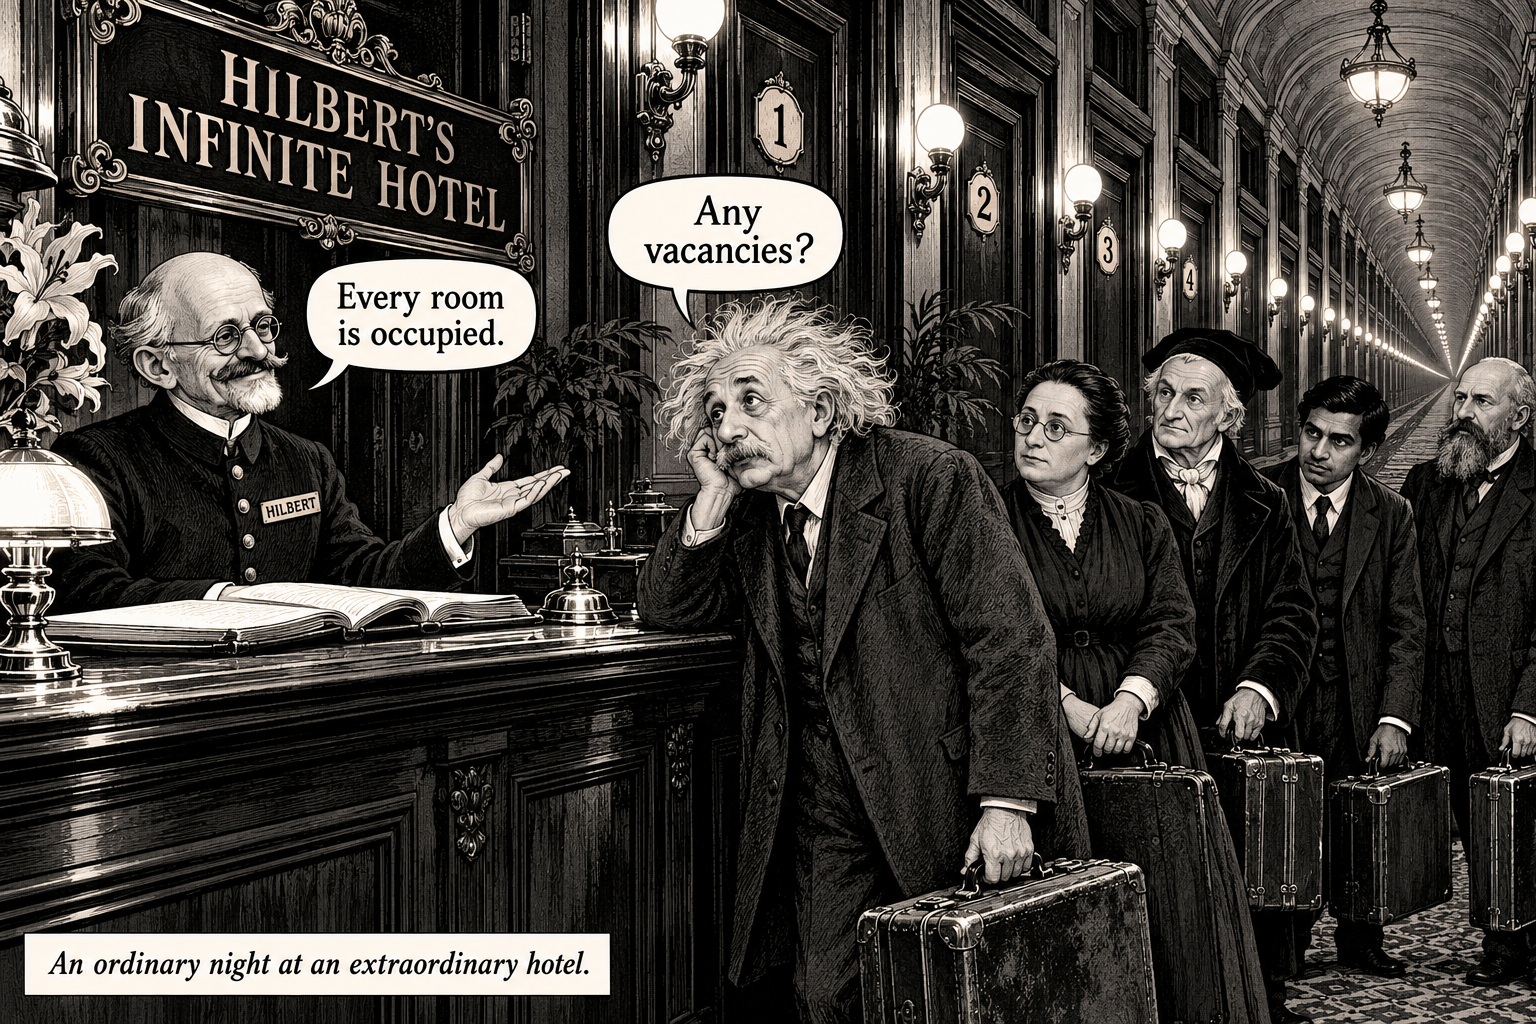
\includegraphics[width=0.8\linewidth]{fig/hotel1}
\end{center}
\end{frame}

\begin{frame}{Hilbert's Infinite Hotel}
\begin{center}
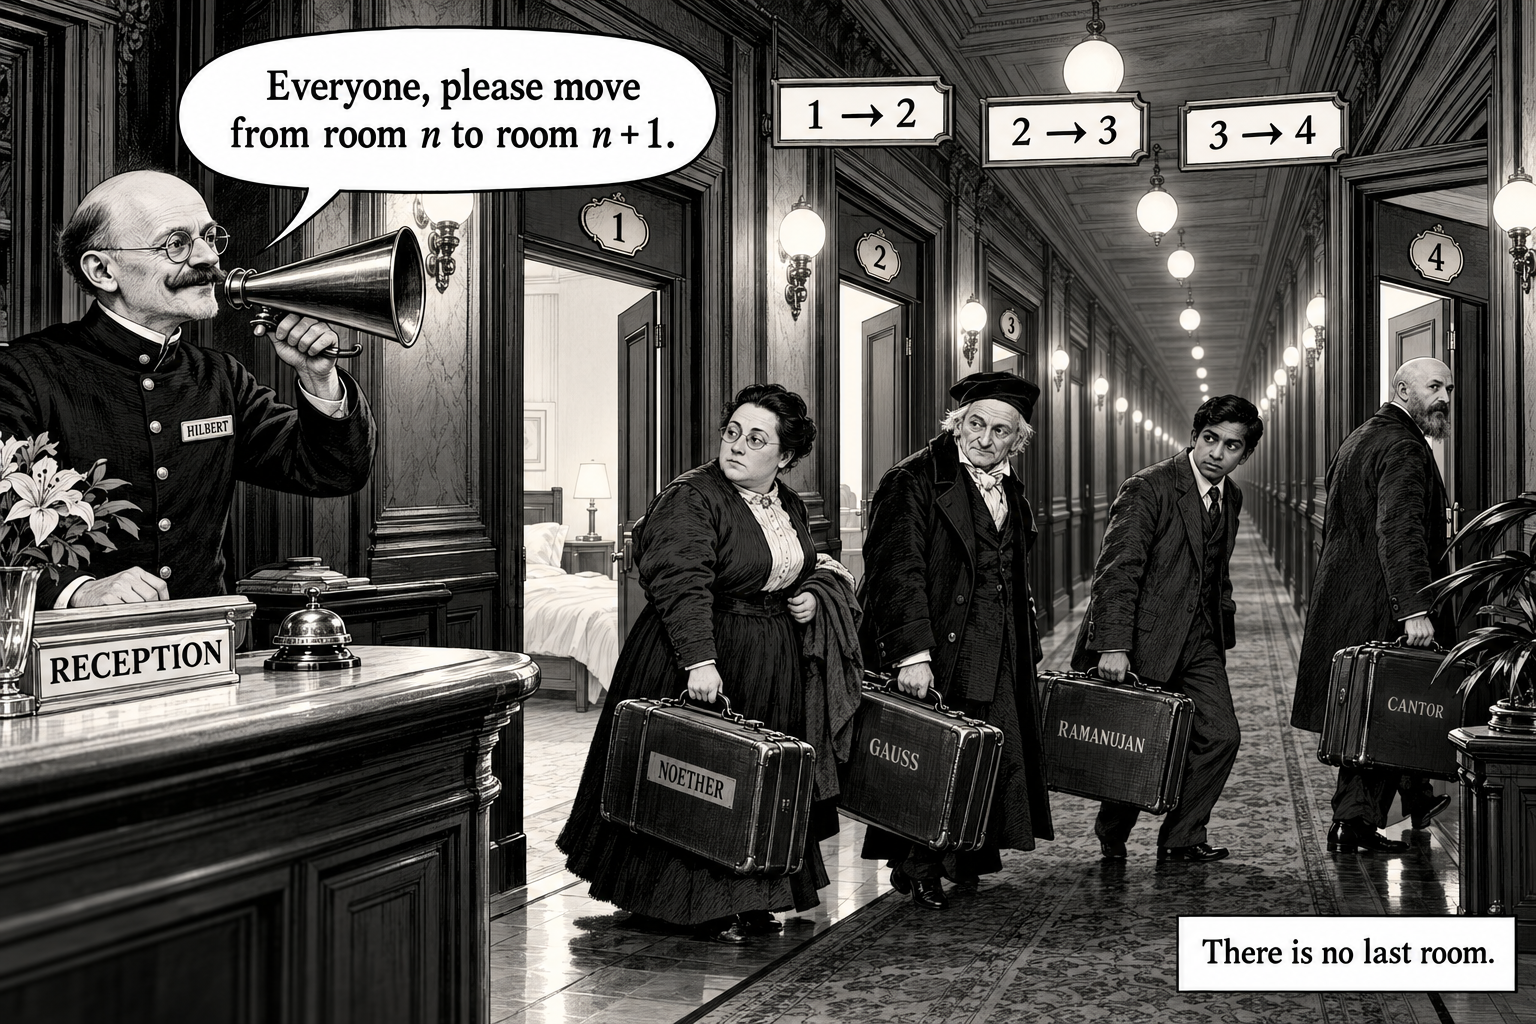
\includegraphics[width=0.8\linewidth]{fig/hotel2}
\end{center}
\end{frame}

\begin{frame}{Hilbert's Infinite Hotel}
\begin{center}
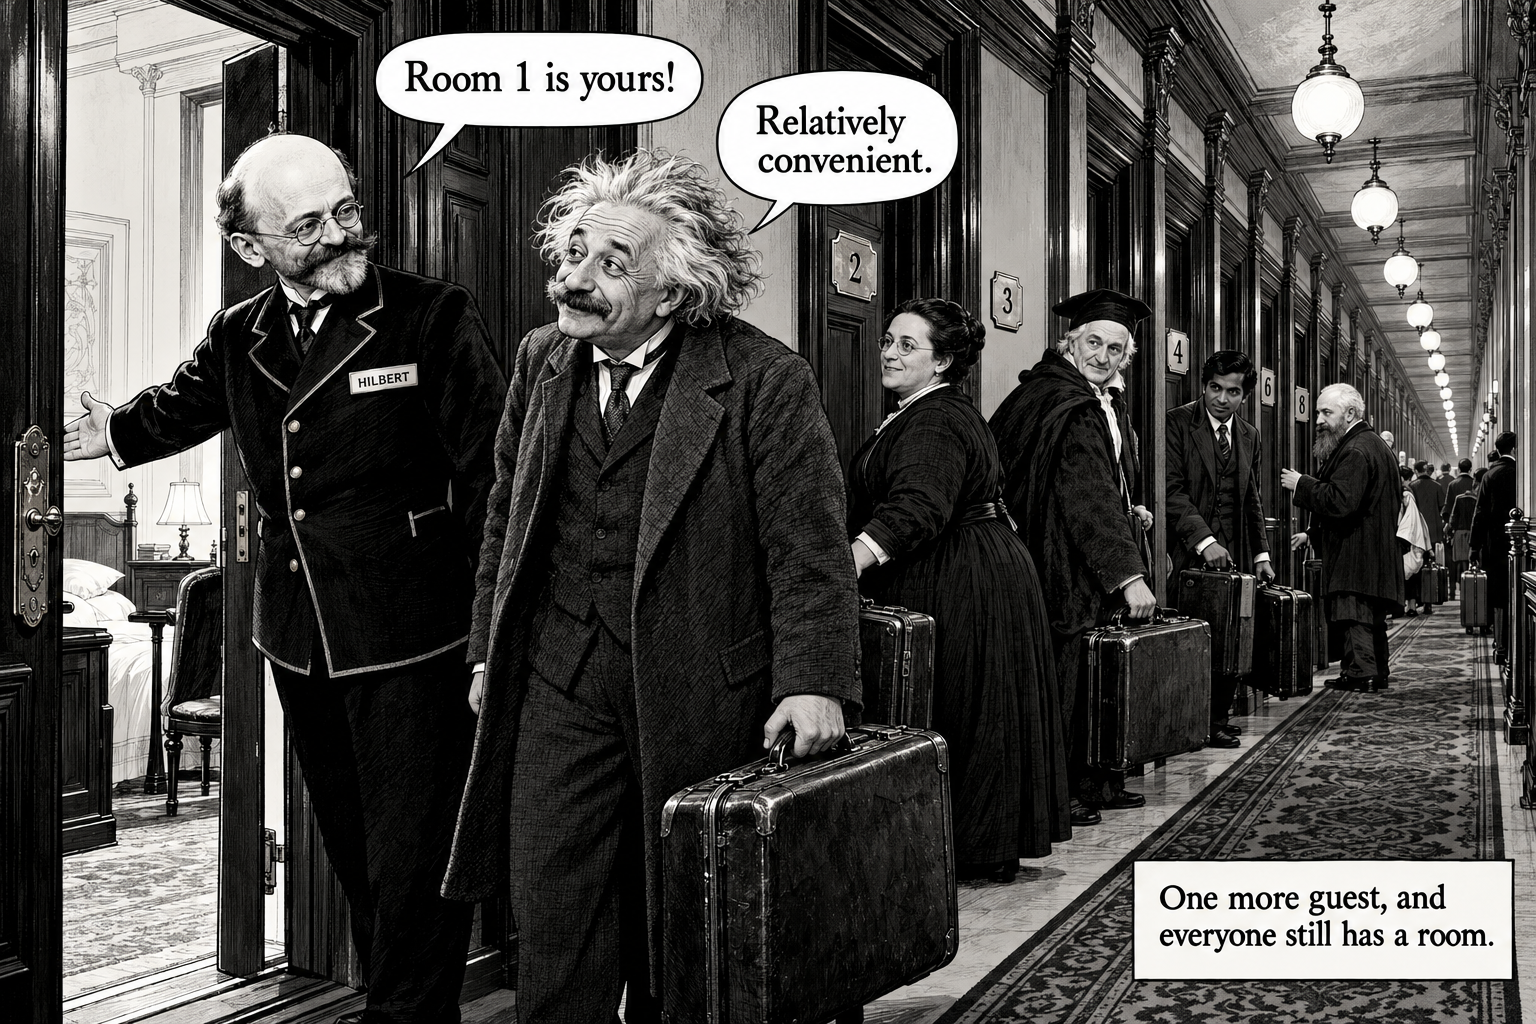
\includegraphics[width=0.8\linewidth]{fig/hotel3}
\end{center}
\end{frame}

\begin{frame}{Hilbert's Infinite Hotel}
Mathematically, we've built a bijection!
$$f: \mathbb N\cup\{0\}\rightarrow\mathbb N$$
$$f(x) = x+1$$
The new guest is $0$.  The old guests are in rooms $2$ and up.  The new guest is in room $1$.
\end{frame}

\begin{frame}{Hilbert's Infinite Hotel}
\begin{block}{Problem}
Later the same night, a bus full of infinitely more guests show up.  Hilbert makes room again!  How does he do it?
\end{block}
\end{frame}

\begin{frame}{Hilbert's Infinite Hotel}
\begin{center}
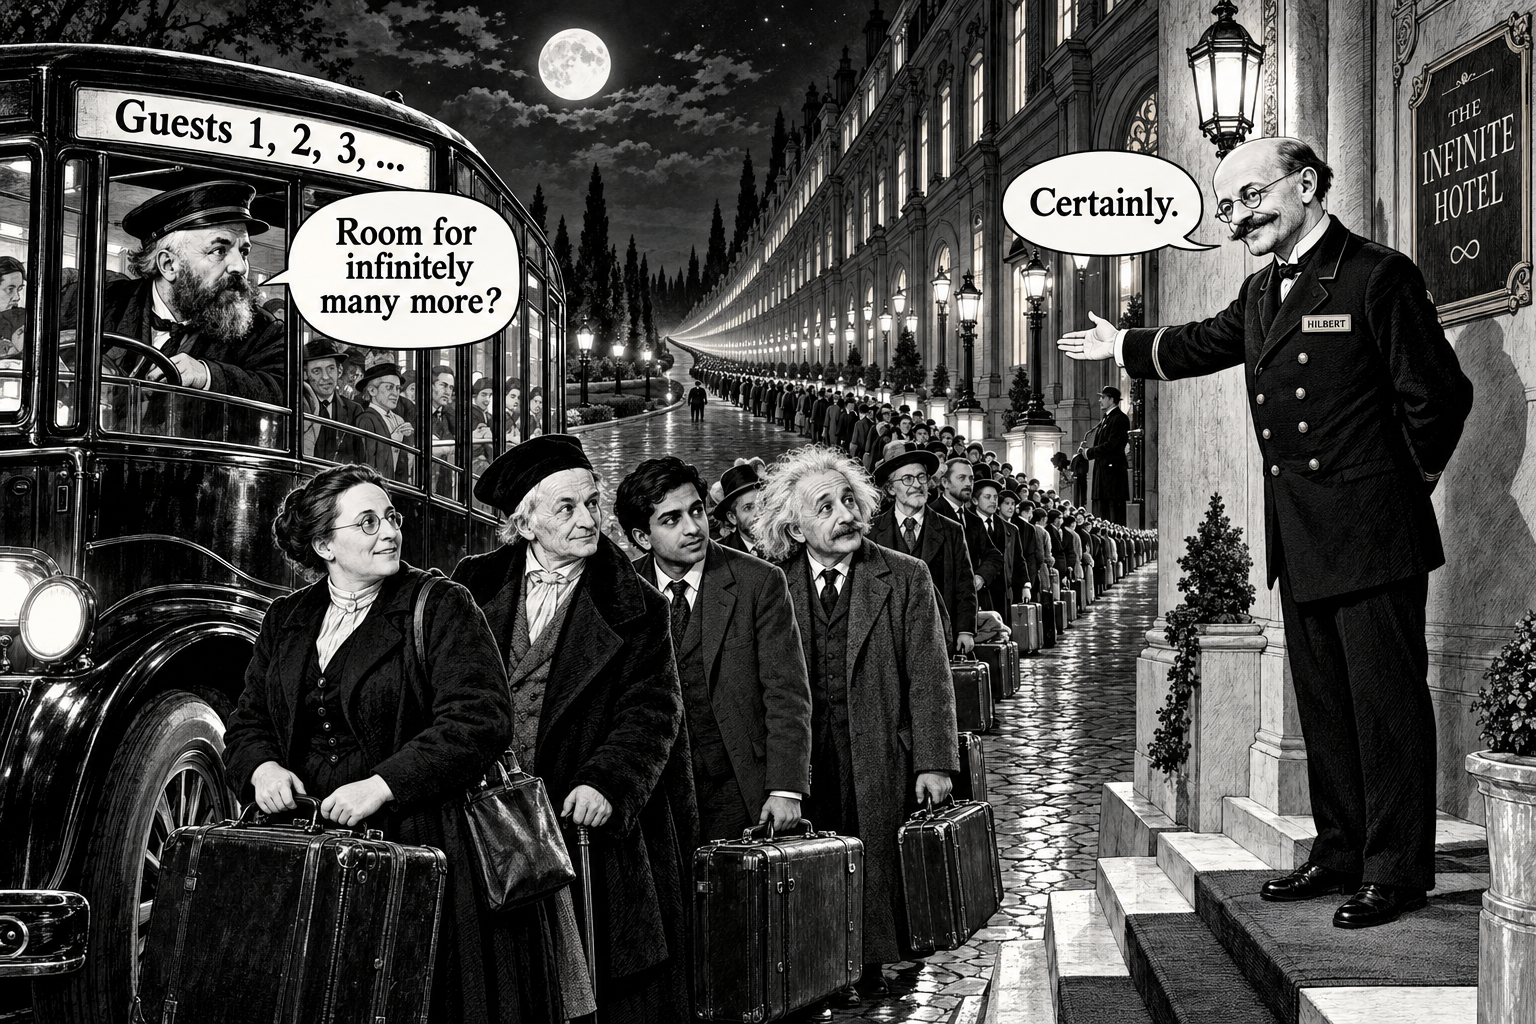
\includegraphics[width=0.8\linewidth]{fig/hotel4}
\end{center}
\end{frame}

\begin{frame}{Hilbert's Infinite Hotel}
\begin{center}
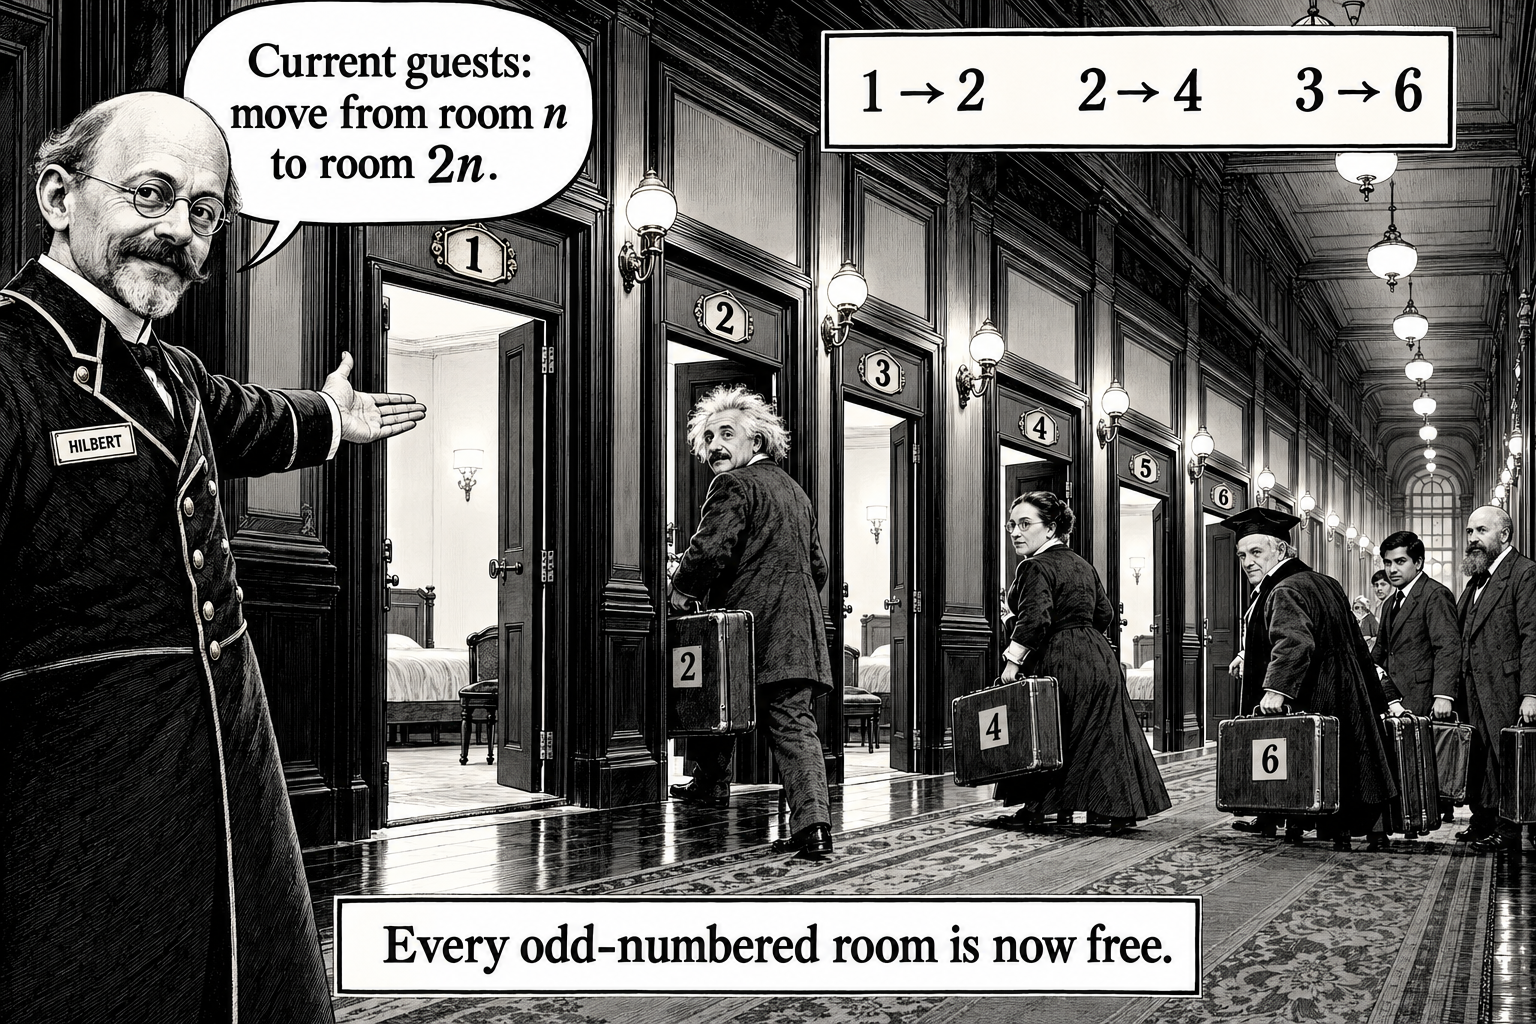
\includegraphics[width=0.8\linewidth]{fig/hotel5}
\end{center}
\end{frame}

\begin{frame}{Hilbert's Infinite Hotel}
\begin{center}
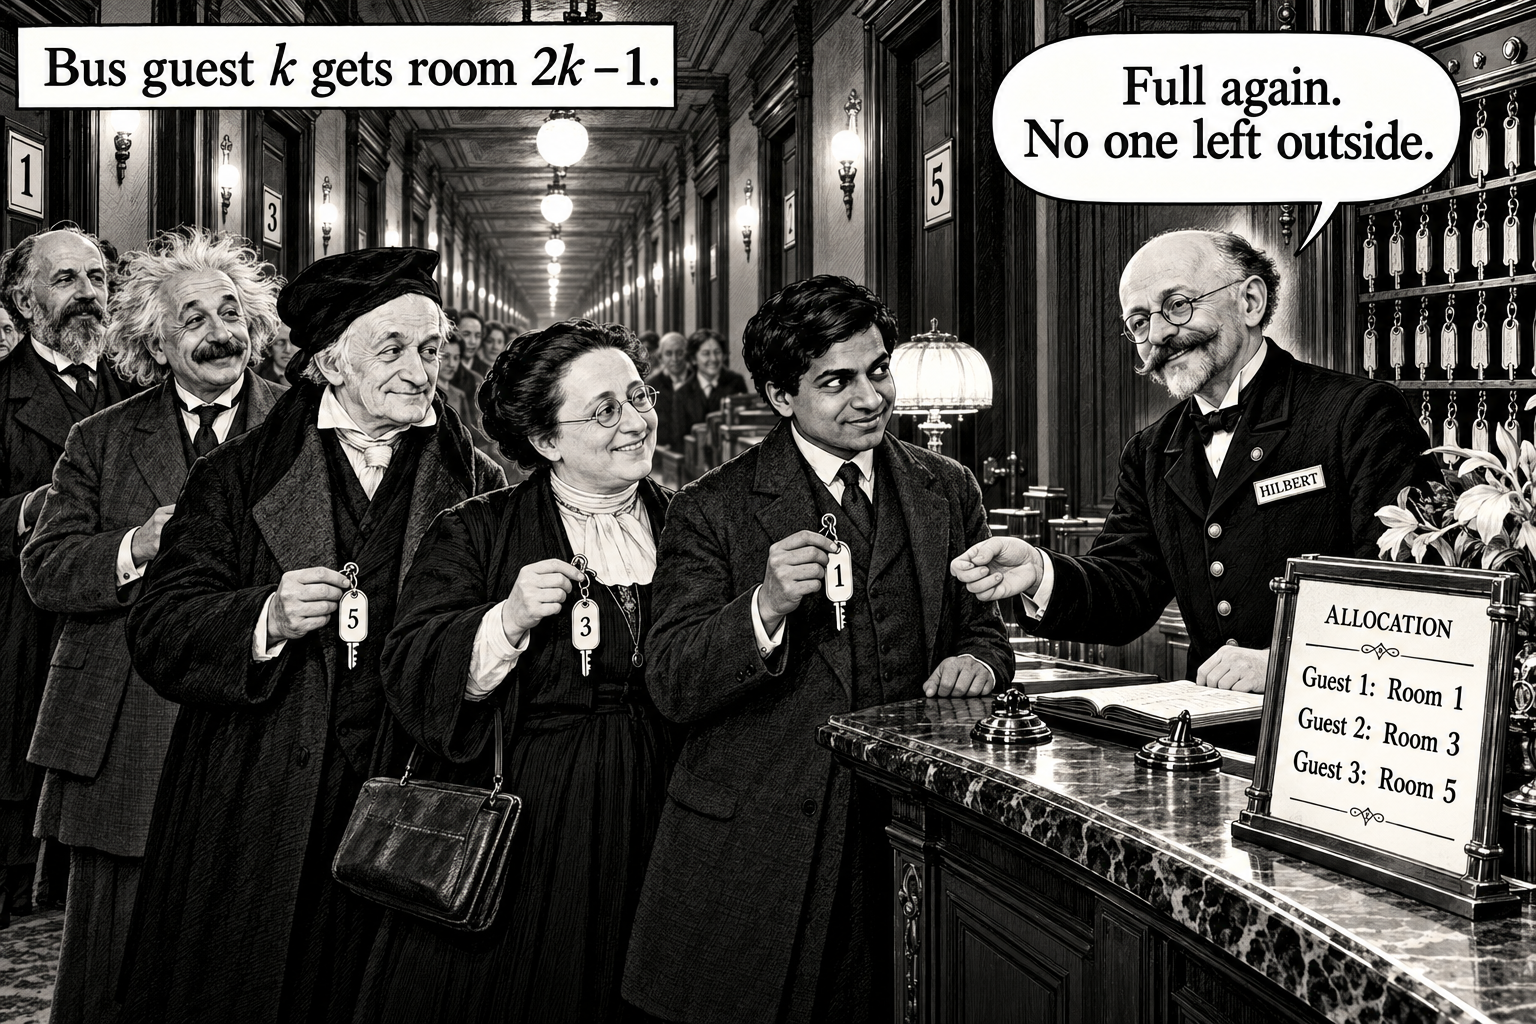
\includegraphics[width=0.8\linewidth]{fig/hotel6}
\end{center}
\end{frame}

\begin{frame}{Hilbert's Infinite Hotel}
Mathematically, we've built another bijection!
$$f: \mathbb Z\rightarrow\mathbb N$$
$$f(x) = \left\lbrace\begin{array}{cc}
2x, & x>0\\
2x+1, & x \leq 0
\end{array}\right.$$
The old guests are in even rooms.  The new guests are in odd rooms.
\end{frame}

\begin{frame}{Hilbert's Infinite Hotel}
\begin{center}
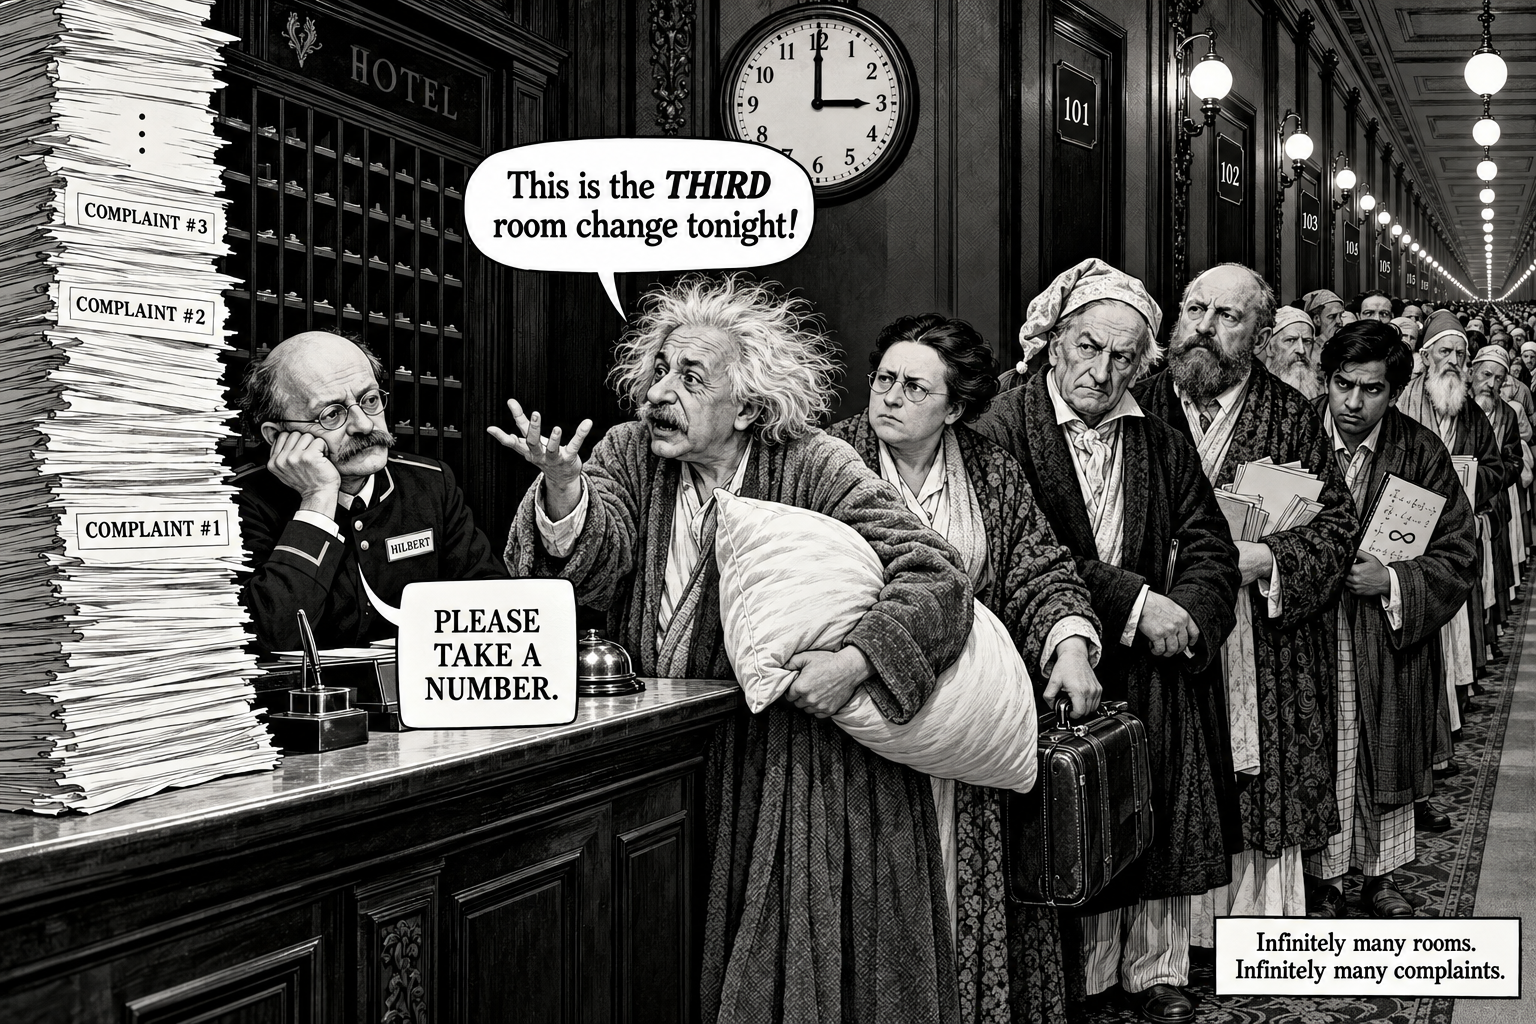
\includegraphics[width=0.8\linewidth]{fig/hotel7}
\end{center}
\end{frame}

\subsection{Wrapping up}

\begin{frame}{Final thoughts}
  \begin{block}{Reflection}
    \begin{itemize}
\pause
      \item  Describe the difference between a relation and a function
      \item  Give an example of a relation which is not a function.  Explain why it isn't.
      \item  Give an example of a function which is surjective but not injective.
    \end{itemize}
  \end{block}
\begin{center}
Submit your responses by \textbf{Tonight!}
\end{center}
\end{frame}


\end{document}


